\section{Theoretical Background in Reinforcement Learning}
Reinforcement learning (RL) is an approach in artificial intelligence for goal-directed learning from interaction and experience. This makes it different from the other approaches in machine learning in which the learner, the decision maker, or the so called agent, is told what to do. In reinforcement learning the agent tries out different actions in order to understand which of them generates the most reward. The reward is a special term in reinforcement learning and describes the goal in a Markov decision process (MDP) model. Roughly speaking, the MDP model would very well characterize the agent’s view of the world, the actions that it can take in the world and its goal.

Machine learning distinguishes supervised from unsupervised learning paradigms by having the supervisor indicating the correct behavior in certain generalized situations for the supervised learning and finding hidden structure in unlabeled data for the unsupervised learning. Reinforcement learning is sometimes classified as an unsupervised learning problem, because it doesn’t make use of labeled data, however it doesn’t look for structure, but tries to maximize the reward. Therefore, reinforcement learning is considered another paradigm in machine learning, according to the opinion and points of the authors R. S. Sutton and A. G. Barto of the book “An introduction to Reinforcement Learning” \cite{Sutton}. The diagram in \Cref{fig:RLandML} illustrates the relationship between machine learning and reinforcement learning.
\begin{figure}[H]
	\centering
	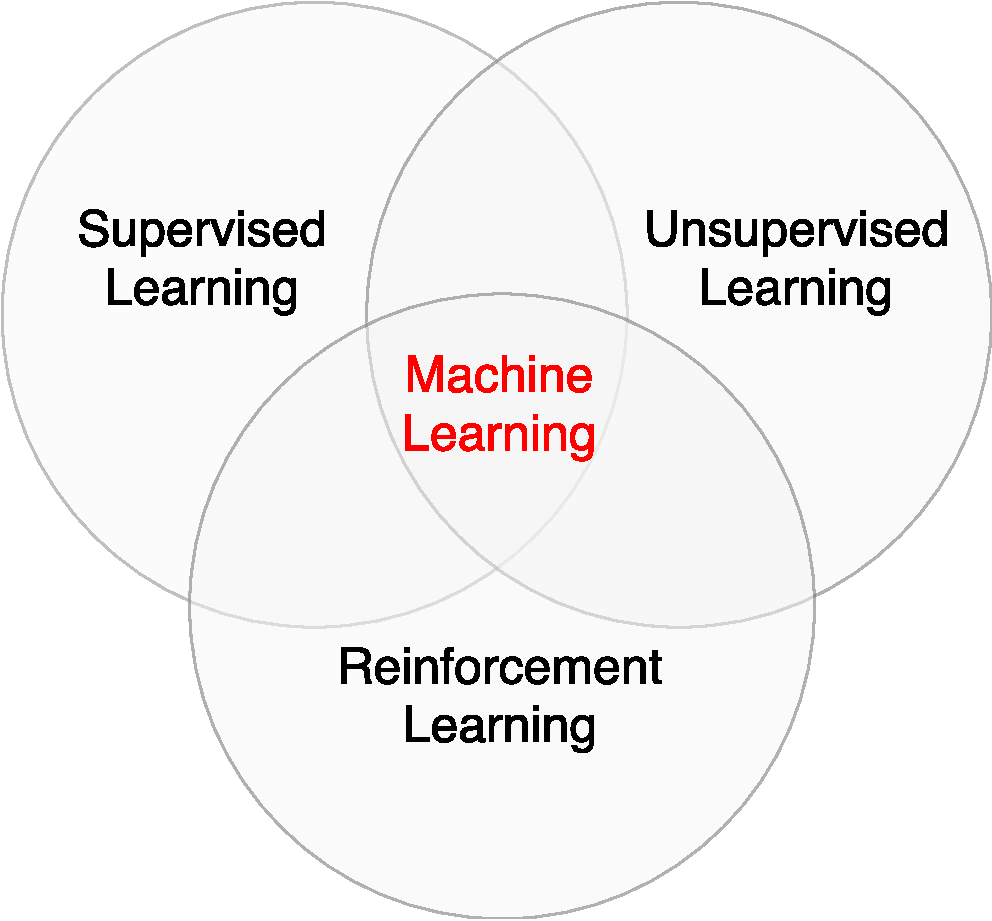
\includegraphics[width=0.7\textwidth]{Figures/RLandML}
	\caption{Reinforcement Learning and Machine Learning}
	\label{fig:RLandML}
\end{figure}
Reinforcement learning considers the problem of planning in real time decision making and the models for prediction related to planning. The interactive goal-directed agent is able to operate in an uncertain set up, make decisions despite uncertainty and predict future events. The agent is not necessarily a robot; it can be any component in a larger system in which it interacts directly with the system and indirectly with the system’s environment. The environment is everything that the agent interacts with, it is the outer world.

There is a special concern in reinforcement learning which is not present in the other machine learning approaches. It is the issue of balancing exploitation of the knowledge that the agent has and exploration of new information in order to improve the current knowledge base.

A variety of different scientific fields intersect with reinforcement learning, especially mathematics, namely, statistics and optimization, which have an important background contribution to the reinforcement learning methods. “For example, the ability of some reinforcement learning methods to learn with parameterized approximators addresses the classical “curse of dimensionality” in operations research and control theory” \cite{Sutton}. The relationship between reinforcement learning and optimization can be exemplified by the idea of maximization of the reward signal. Actually, in reinforcement learning the agent intends to maximize the reward, but not necessarily achieves the maximum. Reinforcement learning is also part of the engineering and computer science subjects. The related algorithms have a close resemblance to the biological brain systems of animals and humans due to the reward factor involved, therefore it also binds with the psychology and neuroscience fields. The diagram in \Cref{fig:RLandOther} illustrates how reinforcement learning relates to other scientific disciplines.
\begin{figure}[H]
	\centering
	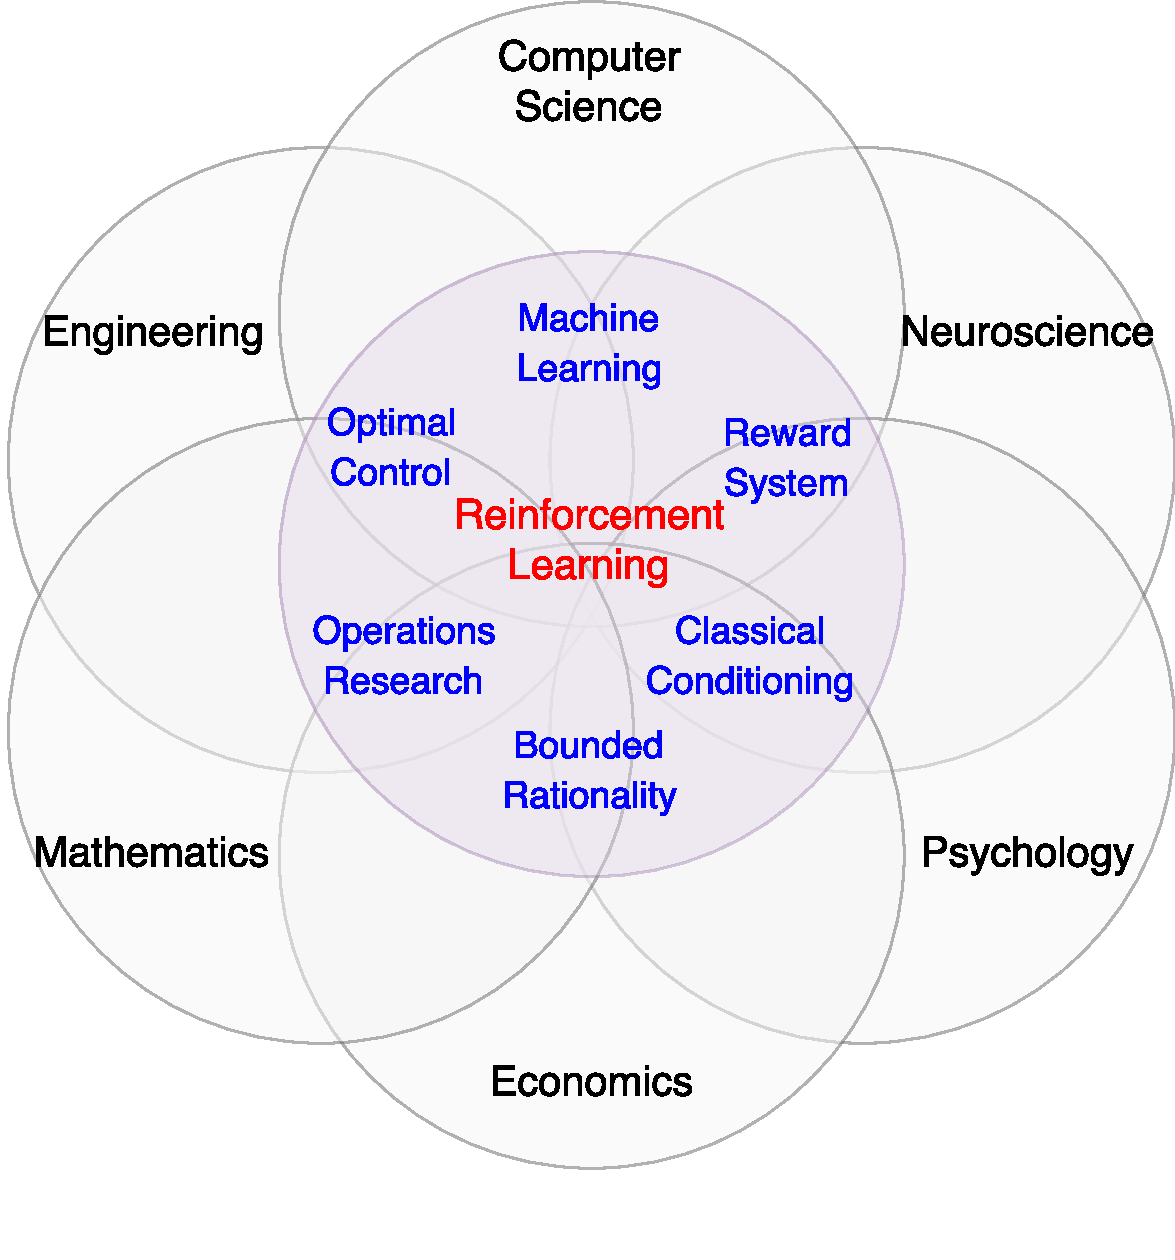
\includegraphics[width=0.7\textwidth]{Figures/RLandOther}
	\caption{Reinforcement Learning and other disciplines}
	\label{fig:RLandOther}
\end{figure}
\subsection{Elements of an RL problem}
A reinforcement learning problem contains at least one of the elements: reward signal, value function, policy, environment model.

The reward signal represents a feedback from the environment as a response to the agent’s behavior in that environment, therefore the agent cannot change the feedback that it receives, but it can behave accordingly so as to maximize the gained reward signals during its lifetime. The “reward signal defines the goal in a reinforcement learning problem” \cite{Sutton}. It serves as a problem definition and as a basis for modifying the policy.

The policy maps states to actions, so that when the agent is in a specific state, it chooses an action based on the defined policy. A policy is enough to describe the behavior of the agent and therefore, it is the core of reinforcement learning.

The value function provides values for judging about the quality of a state based on the estimated maximum reward it can yield in the long run, in contrast with the reward which expresses only the immediate advantage of being in a specific state.

The model is a representation of the environment’s behavior. In a model-free reinforcement learning (trial-and-error) problem the agent cannot plan its future, because it doesn’t have a model basis, whereas in mode-based problems the agent can plan its future actions based on the environment’s modelled behavior and expected rewards in certain states.
\subsection{Markov Decision Processes in RL}
The general reinforcement learning problem formulation has the format of a finite MDP. The interaction between the agent and environment happens at each time step of a sequence of discrete time steps, $t=0,1,2,3,...$, where at each time step $t$ the agent receives a representation of the world - a state, $S_{t}\in S$, from a set of possible states $S$, selects an action $A_{t}$ from a set of possible actions $A(S_{t})$ for the state $S_{t}$ by implementing a policy $\pi_{t}$, where $\pi_{t}(a|s)$ is the probability that $A_{t}=a$ if $S_{t}=s$, and in the next time step $t+1$ the agent receives a reward signal $R_{t+1}\in R$ from the environment ending up in a new state $S_{t+1}$ \cite{Sutton}. The diagram in \Cref{fig:AgentEnv} illustrates the interaction between the agent and the environment.
\begin{figure}[H]
	\centering
	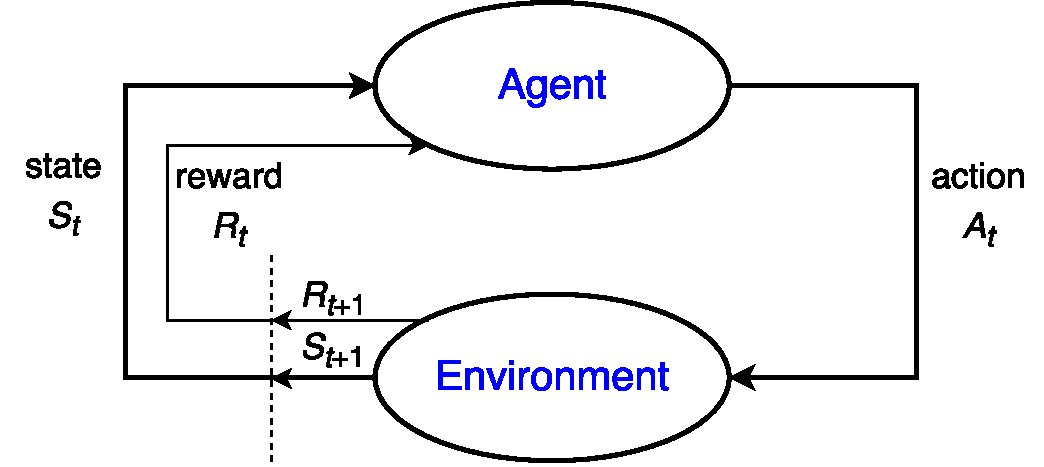
\includegraphics[width=0.7\textwidth]{Figures/Agent-EnvironmentInteraction}
	\caption{Agent - environment interaction}
	\label{fig:AgentEnv}
\end{figure}
Reinforcement learning methods provide ways to adjust the policy based on the accumulated experience with the goal of maximizing the total cumulative reward in mind. An example for representing the goal in a reinforcement learning problem like that of making a robot learn to walk would be by giving a reward on each time step proportional to the robot's forward motion. “The reward signal is your way of communicating to the robot \textit{what} you want it to achieve, not \textit{how} you want it achieved” \cite{Sutton}.

A formal definition of the cumulative reward received in the long run is expressed by the expected return $G_{t}$, which is a function of rewards sequence $R_{t+1},R_{t+2},...,R_{T}$ received after the time step $t$, where $T$ is the last time step. In order to express the return more conveniently the concept of \textit{discounting} is introduced, which determines the current value of the future rewards. The formula generalized for both episodic and continuing tasks is the following: 
\begin{equation}
G_{t}=R_{t+1}+\gamma R_{t+2}+\gamma ^2R_{t+3}+...=\sum_{k=0}^{T-t-1}\gamma ^kR_{t+k+1}, 
\end{equation}
where $\gamma$ is the discount rate, $0\leq \gamma\leq1$. In the case of episodic tasks where there is a terminal state after some time steps, $\gamma=1$. For the cases in which the process is continuous and the final step is infinite, $T=\infty$. 

With the discounting factor, the reward received after $k$ time steps has the value "$\gamma ^{k-1}$ times what it would be worth if it were received immediately" \cite{Sutton}. In the extreme point where $\gamma=0$, it is said that the agent is myopic, because it only maximizes over the immediate rewards and not the future rewards, whereas if $\gamma$ is closer to $1$ the agent is farsighted and sees far into the future considering the future rewards when picking actions.

The \textit{state} that has the Markov property represents all the useful information in order to make a sufficient statistic for the future. With Markov states we have the best possible basis for choosing action \cite{Sutton}. The environment's feedback at time step $t+1$ after a particular action was taken at time step $t$ depends on the events happened before. If the state has the Markov property instead, then the feedback of the environment depends only on that state, because that state represents all the previous events. In this case the one step environment dynamics of a finite MDP can be expressed by the following formula:
\begin{equation}\label{psrsa}
p(s',r|s,a)=Pr\left \{ S_{t+1}=s',R_{t+1}=r|S_{t}=s,A_{t}=a \right \}
\end{equation}
Based on the formula presented in (\ref{psrsa}) we can also compute the expected rewards for state-action pairs \cite{Sutton},
\begin{equation}
r(s,a)=\mathop{{}\mathbb{E}}\left [ R_{t+1}|S_{t}=s,A_{t}=a \right ]=\sum_{r\in R}r\sum_{s'\in S}p(s',r|s,a)
\end{equation}
the \textit{state-transition probabilities}
\begin{equation}
p(s'|s,a)=Pr\left \{ S_{t+1}=s'|S_{t}=s,A_{t}=a \right \}=\sum_{r\in R}p(s',r|s,a)
\end{equation}
and the expected rewards for state-action-next-state triples,
\begin{equation}
r(s,a,s')=\mathop{{}\mathbb{E}}\left [ R_{t+1}|S_{t}=s,A_{t}=a,S_{t+1}=s' \right ]=
\frac{\sum_{r\in R}rp(s',r|s,a)}{p(s'|s,a)}
\end{equation}
Value functions estimate how good it is to be in a specific state given the expected return and the policy.

The \textit{state-value function} for policy $\pi$, $v_{\pi }$ expresses the expected value of a random variable given the followed policy $\pi$ at any time step $t$:
\begin{equation}
v_{\pi }(s)=\mathop{{}\mathbb{E}_{\pi}}\left [G_{t}|S_{t}=s \right ]=\mathop{{}\mathbb{E}_{\pi}}\left [ \sum_{k=0}^{\infty}\gamma ^kR_{t+k+1} |S_{t}=s\right ]
\end{equation}

The \textit{action-value function} for policy $\pi$, $q_{\pi }$ is the value of taking an action $a$ in a state $s$ while following the policy $\pi$:
\begin{equation}
q_{\pi }(a,s)=\mathop{{}\mathbb{E}_{\pi}}\left [G_{t}|S_{t}=s,A_{t}=a \right ]=\mathop{{}\mathbb{E}_{\pi}}\left [ \sum_{k=0}^{\infty}\gamma ^kR_{t+k+1} |S_{t}=s,A_{t}=a\right ]
\end{equation}

Value functions have the property of being expressed recursively. The recursive representation is actually the \textit{Bellman equation} and it's solution is the value of $v_{\pi }$. It is like a look ahead procedure, where the value of a current state is evaluated by looking ahead at the values that future states can offer. "The Bellman equation averages over all the possibilities, weighting each by its probability of occurring. It states that the value of the start state must equal the (discounted) value of the expected next state, plus the reward expected along the way" \cite{Sutton}:
\begin{equation}\label{StateValueFunction}
v_{\pi }(s)=\mathop{{}\mathbb{E}_{\pi}}\left [G_{t}|S_{t}=s \right ]=\sum_{a}\pi(a|s)\sum_{s',r}p(s',r|s,a)\left [ r+\gamma v_{\pi }(s') \right ]), \forall s\in S
\end{equation}
The Bellman equation represents the basis of different ways of computing, approximating, and learning $v_{\pi }$ \cite{Sutton}.

In finite MDPs, an \textit{optimal policy} $\pi_{*}$ is the policy for which its expected return for all the states is greater than or equal to the expected return of all the other policies. There can be many policies that are optimal due to their \textit{state-value function}, which evaluates the same for all the optimal policies:\begin{equation}
v_{*}(s)=\max_{\pi}v_{\pi}(s), \forall s\in S
\end{equation}

Analogically, the \textit{optimal action-value function} is formed:
\begin{equation}
q_{*}(s,a)=\max_{\pi}q_{\pi}(s,a), \forall s\in S , a \in A(s)
\end{equation}

The \textit{Bellman optimality equation} for $v_{*}$ is the value of a state on the optimal policy basis, which is the same as the expected return of the best action for that state \cite{Sutton}:
\begin{equation}\label{BellmanOptimalityVstar}
\begin{split}
v_{*}(s)&=\max_{a \in A(s)}q_{\pi*}(s,a) \\
&=\mathop{{}\mathbb{E}}\left [ R_{t+1} + \gamma v_{*}(S_{t+1})|S_{t}=s, A_{t}=a  \right ] \\
&=\max_{a \in A(s)}\sum_{s',r}p(s',r|s,a)\left [ r+\gamma v_{*}(s') \right ]
\end{split}
\end{equation}

And the \textit{Bellman optimality equation} for $q_{*}$ is the following:
\begin{equation}\label{BellmanOptimalityQstar}
\begin{split}
q_{*}(s,a)&=\mathop{{}\mathbb{E}}\left [ R_{t+1} + \gamma \max_{a'}q_{*}(S_{t+1},a')|S_{t}=s, A_{t}=a  \right ] \\
&=\sum_{s',r}p(s',r|s,a)\left [ r+\gamma\max_{a'}q_{*}(s',a') \right ]
\end{split}
\end{equation}

The Bellman optimality equation generates a system of $N$ nonlinear equations, where $N$ is the number of states. It can be simply solved by applying some nonlinear methods when the system dynamics ($p(s',r|s,a)$) are known. The solution to the Bellman optimality equation helps in defining the optimal policy; e.g. one can, at any state, choose the action that corresponds to the maximum return, which is also valid in the long term, because the values take into account the reward consequences of all possible future behavior options \cite{Sutton}. In the case of the action-value pairs, if the system's dynamics are unknown, then the actions would still be optimal, because the agent would choose the actions that would maximize $q_{*}$.

\subsection{Insight into the Solution Methods of RL}
The solution methods for the reinforcement learning problem can be divided into two groups, \textit{tabular} and \textit{approximate}. The tabular solution methods find exact, optimal solutions and are more suitable when the states and actions space is rather small, while the approximate solution methods provide approximate solutions and it is applicable to large spaces problems.

The process of \textit{generalized policy iteration} (GPI) provides a good way of getting insight into the methods of RL. GPI employs a sequence of interleaved policy evaluations and policy improvements, where the given policy is evaluated, for example, by computing it's value function, and the policy is improved by using the value function. This process is proven to converge to an optimal policy and value function for the classical dynamic programming methods. GPI represents the way that almost all RL methods work. The \Cref{fig:GPI} illustrates the process better.
\begin{figure}[H]
	\centering
	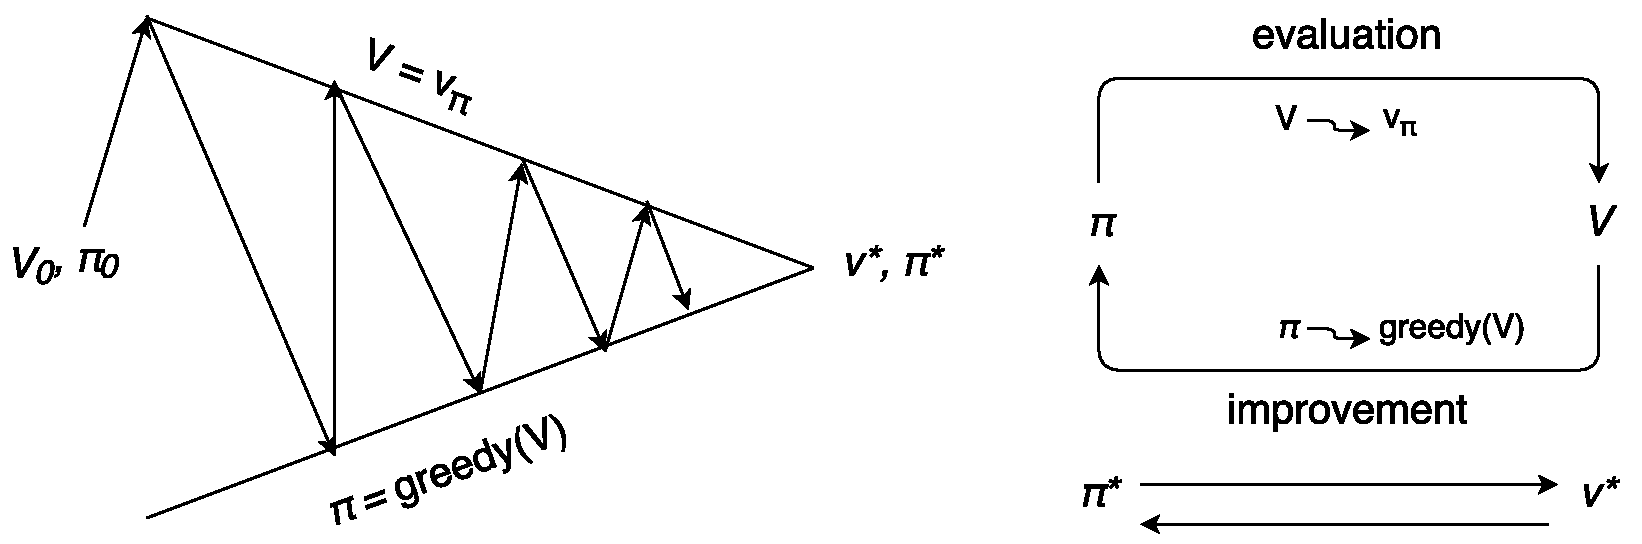
\includegraphics[width=0.9\textwidth]{Figures/GPI}
	\caption{Generalized Policy Iteration}
	\label{fig:GPI}
\end{figure}
Another way of presenting the GPI is in terms of \textit{prediction} and \textit{control}. The prediction problem is referring to policy evaluation or the estimation of $v_{\pi}$ for a given policy $\pi$, whereas the control problem is referring to the actual optimal policy $\pi_{*}$ seeking.

The relevant notions for describing the methods of RL are \textit{backup} and \textit{bootstrap}. A \textit{full backup} updates a state's value on the basis of the next states estimated values. \textit{Bootstrapping} refers to the idea of updating estimates based on other estimates.

Usually, the RL solution methods vary in the way they approach the prediction and control problems, and also in whether they need a model of the environment or they use bootstrapping.

\subsection{Tabular solution methods}
The tabular solution methods include three important classes of methods for solving the finite MDP: \textit{Dynamic Programming} (DP), \textit{Monte Carlo} (MC) and \textit{Temporal-Difference} (TD) learning. These methods will be generally presented in the following pages.

\subsubsection{Dynamic Programming}
Dynamic programming uses the Bellman optimality equations \ref{BellmanOptimalityVstar} and \ref{BellmanOptimalityQstar} as update functions for \textit{policy iteration}, which yields a sequence of monotonically increasing value functions and policies: ${\pi}_{0}\overset{E}{\rightarrow}v_{{\pi}_{0}}\overset{I}{\rightarrow}{\pi}_{1}\overset{E}{\rightarrow}v_{{\pi}_{1}}\overset{I}{\rightarrow}{\pi}_{2}\overset{E}{\rightarrow}...\overset{I}{\rightarrow}{\pi}_{*}\overset{E}{\rightarrow}v_{*}$, where $E$ stands for evaluation and $I$ - for improvement. That is, an arbitrary fixed policy is evaluated by computing it's state-value function and is improved by computing it's state-action value function. If the state-action value function of choosing an action $a \neq \pi(s)$ is greater than the state-value function $v_{\pi}(s)$, then the policy is changed to a new policy. The formula for getting a new policy is given by \ref{PolicyImprovement}:
\begin{equation}\label{PolicyImprovement}
\begin{split}
\pi'&=\arg\!\max_{a}q_{\pi}(s,a)\\
&=\arg\!\max_{a}\mathop{{}\mathbb{E}}\left [ R_{t+1} + \gamma v_{\pi}(S_{t+1})|S_{t}=s, A_{t}=a  \right ] \\
&=\arg\!\max_{a}\sum_{s',r}p(s',r|s,a)\left [ r+\gamma v_{\pi}(s') \right ]
\end{split}
\end{equation}

Unlike the DP methods, the Monte Carlo and the temporal-difference solution methods don't require the model parameters to be known in advance, meaning that no previous knowledge about the environment is needed and that the agent learns exclusively from it's \textit{experience} (sampled states, actions, rewards). The MC method doesn't bootstrap, whereas TD does use bootstrapping, like the DP methods.

\subsubsection{Monte Carlo}
Monte Carlo differs from DP in the way it handles the prediction problem. It uses averages over the sampled returns from a specific state on episode-by-episode basis in order to learn over multiple observed returns the value function, whereas in DP the value function was computed from the knowledge of the MDP. The policy evaluation is performed by computing the value of the state-action pairs for the visited states over an episode. The policy improvement is performed by adjusting the policy closer to the action with the maximal value for a specific state.

Because MC doesn't make all the possible actions, it is required to employ some kind of guarantee for exploration. This can be achieved by assigning nonzero probabilities for all the actions in order to make sure they are going to be picked eventually. This is called \textit{exploring starts}. A better approach are the \textit{on-policy} and \textit{off-policy} methods. 

On-policy methods have probabilities greater than zero for all their actions, meaning that they have \textit{soft} policies. The policies in on-policy methods become closer to an optimal deterministic policy in time. The exploring starts is an example of on-policy method. Another example would be an $\epsilon$-greedy policy where the best action is chosen with the probability $1-\epsilon$ and, sometimes, another random action is chosen with the probability $\epsilon$.

Off-policy methods use 2 policies: a \textit{target policy} $\pi$, which is a deterministic policy, like the one presented in the on-policy methods, and a \textit{behavior policy} $\mu$, which is stochastic in states and generates data by exploring. Both policies have non zero probabilities that ensures the coverage property. Off-policy methods can be implemented with \textit{importance sampling} technique. The importance sampling technique computes an importance sampling ratio based on the relative probabilities of the returns' trajectories from both policies and it is used for weighting the returns for learning the value function.

\subsubsection{Temporal Difference}\label{Temporal Difference}
Temporal Difference differs from DP also in the way it handles the prediction problem. TD makes an estimate of the value function after each time step by sampling expected values and using current value estimates. Therefore, TD is a combination of MC sampling and DP bootstrapping. The simplest TD method is also called \textit{TD(0)}. The update function for TD(0) \ref{PolicyEvaluationTD0} is the following:
\begin{equation}\label{PolicyEvaluationTD0}
V(S_{t})\leftarrow V(S_{t})+\alpha \left [ R_{t+1}+\gamma V(S_{t+1})-V(S_{t}) \right ]
\end{equation}
If we compare the MC target with the TD target, the MC target has $G_{t}$ instead of the immediate reward and the value estimate of the next state. The square brackets represents the TD error, or the MC error in the MC update function. An important observation is that the sum of the time steps TD errors gives an episode of MC error.

For solving the control problem with TD(0) and on-policy methods, action-value functions are used instead of the value function that we've just seen. A "transition from one action-state pair to another" \cite{Sutton} yields a quintuple of the form $(S_{t}, A_{t}, R_{t+1}, S_{t+1}, A_{t+1})$, \textit{Sarsa}, which is the name of the algorithm. Therefore, for evaluating the policy, an estimation of the $q_{\pi}$ is required and for improving the policy, $\pi$ is greedily adjusted closer to it's $q_{\pi}$.

An notable off-policy TD(0) algorithm is \textit{Q-learning}. It is an off-policy method because it learns the optimal action-value function $q_{\pi*}$ independent of the policy. The action is picked greedily according to the estimated $Q$ but the $Q$ is updated based on the action that produces maximal value. 

A slight change into the update function of $Q$ would lead us to the \textit{Expected Sarsa} algorithm. The change is that instead of maximizing over the next action-value pairs, the expected return is taken, which considers the probabilities of making those actions according to the current policy. Expected Sarsa is a better algorithm in comparison with Sarsa and Q-learning.

The MC and TD methods are extended into more complicated and powerful forms to achieve better performance, but the essence of these methods perpetuates in all the other algorithms. An idea about combining these two methods would be to unify them under \textit{n-step} algorithms instead of the extreme one time step in TD(0) and a whole episode in MC, or perform additions of other features like eligibility traces and model learning.
	
\subsection{Approximate solution methods}\label{Approximate solution methods}
The approximate solution methods are an extension to the tabular solution methods for huge states spaces problems. In this type of problems, the goal is to find a good approximate solution under the condition of restricted computational resources. Because almost every visited state is seen for the first time, every state being so unique, the agent needs to be able to make sense of it and, therefore, usefully generalize the information it gets. This is possible thanks to function approximation. “Function approximation is an instance of supervised learning, the primary topic studied in machine learning, artificial neural networks, pattern recognition, and statistical curve fitting” \cite{Sutton}.

The value function is represented by a function of a weights vector instead of a table. The approximated value function looks like $\hat{v}(s,\theta)\approx v_{\pi}(s)$, which can be translated into words as the approximated value of a state $s$ given the weights vector $\theta$. The value function can be an artificial neural network with multiple layers where the weights are adjusted and learned. A single adjustment of the weights would change the value appreciation for all the states. This process is difficult to follow and track, but it is more powerful. This would create the necessary \textit{generalization} for the agent to learn from it and apply knowledge in multiple similar, but different states.

With function approximation different supervised machine learning methods can be applied to simulate outputs for a set of inputs. The estimated value of a state $s$ should look more like a number $g$ and this relation $s \mapsto g$ can be used as a training example for supervised learning that would learn to predict values for other states. $s \mapsto g$ is referred to as a back-up, where $s$ is the state backed-up and $g$ is the backed-up value or target. For example, the target in MC methods is the return $G_{t}$, so the back-up is $S_{t} \mapsto G_{t}$, whereas the back-up in TD(0) is $S_{t} \mapsto R_{t+1}+\gamma\hat{v}(S_{t+1}, \theta_{t}) $.

Some common way of doing function approximation is based on gradient principles. For any $\theta$ the function approximator can not exactly represent all the states and examples, therefore the idea is to find a balance - a weights vector that would, as close as possible, represent all the states. A performance measure could be defined by the \textit{mean squared value error} (MSVE) shown below (\Cref{MSVE}). The error represents the squared difference between the estimated value $\hat{v}(s,\theta)$ and the actual value $v_{\pi}(s)$, whereas the $d(s)$ represents the weight or the distribution of the error for a state $s$. The goal would become the minimization of MVSE.
\begin{equation}\label{MSVE}
MVSE(\theta)=\sum_{s\in S} d(s) \left [ v_{\pi}(s) - \hat{v}(s,\theta) \right ]^{2}
\end{equation}

For each training example the \textit{Stochastic Gradient Descent} (SGD) method would update the weights so that they minimize the error in that example:
\begin{equation}\label{SGD}
\theta_{t+1}=\theta_{t}+\alpha \left [ v_{\pi}(S_{t}) - \hat{v}(S_{t},\theta_{t}) \right ]\nabla\hat{v}(S_{t},\theta_{t})
\end{equation}
In the MC method, the target is an unbiased estimate of $v_{\pi}(s)$, therefore the SGD would be a good choice to be applied, because it would converge to a locally optimal solution for the value function. In the bootstrapping cases, however, SGD is not the best choice, because the targets usually depend on the weights vector that is changing and causing the targets to be biased. These methods are called \textit{semi-gradient} methods instead, and they converge in the linear case.

Linear methods have feature vectors $\phi(s)$ that represent the state. The inner product between the feature vector $\phi(s)$ and the weights $\theta$ makes up the function approximation $v_{\pi}(s,\theta)$. In such a situation the SGD method can be applied and get an even simpler form of weights update. This is proven to converge to a global optimum, including for the MC linear function approximation version and the semi-gradient TD(0) with an additional theorem.

\subsubsection{Artificial Neural Networks}
Nonlinear methods for function approximation involve \textit{artificial neural networks} (ANNs). ANNs are the product of inspiration from the neural networks in the brains of animals and humans. Their properties and functionality have been successfully replicated in ANNs. An ANN is a layered structure of neurons which has minimum one input layer and one output layer. Each layer has a number of units (neurons) that are connected to the units in another layer. The connections are assigned weights that are used for the unit's \textit{activation}. In order to perform activation, a weighted sum of it's inputs is computed at each unit and then passed to an activation function to produce output. There are different activation functions, though, and the choice depends on the type of problem.

In dependence of the structure of the network, there are different types of ANNs. For example, a simple case of \textit{feedforward} ANN without any loops, with an input layer of 4 units, 2 hidden layers, and an output layer with 2 units is presented in the \Cref{fig:feedforward}:
\begin{figure}[H]
	\centering
	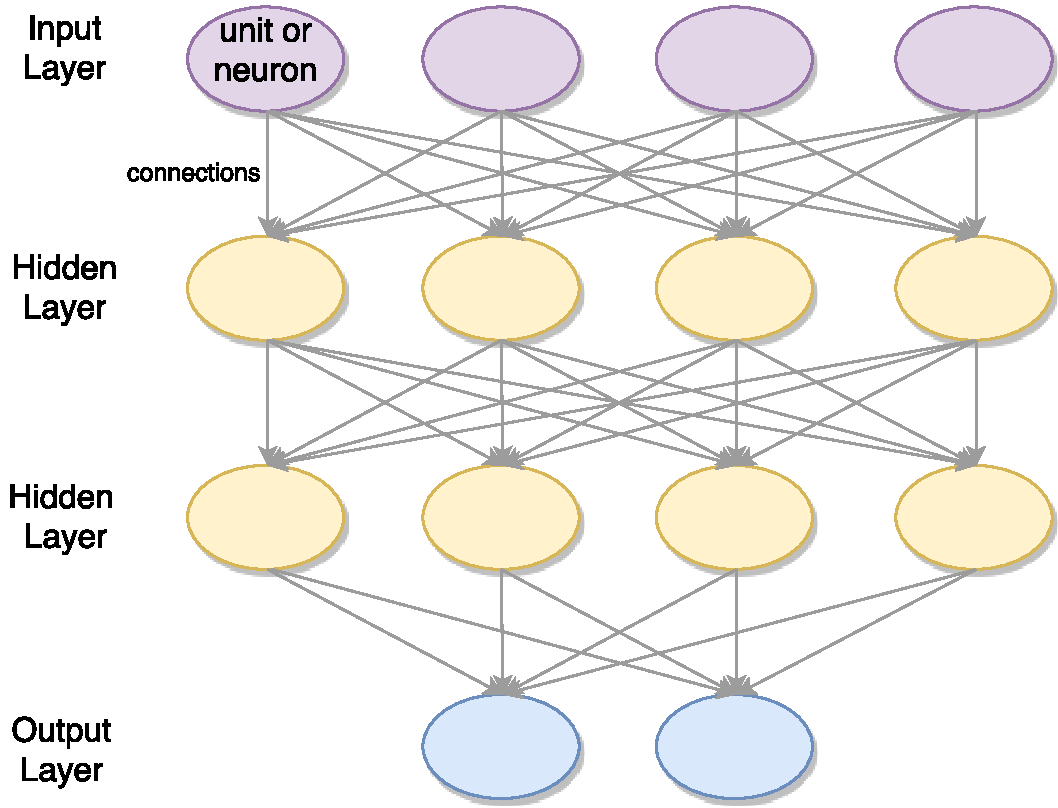
\includegraphics[width=0.7\textwidth]{Figures/Feedforward}
	\caption{Feedforward ANN}
	\label{fig:feedforward}
\end{figure}
Some ANNs can be called \textit{deep}. This qualifier describes the networks that have many hidden layers, precisely more than two. More hidden layers would compute more abstract representations of the input data, which means richer features. Deep ANNs are harder to train, but they are more powerful, and are especially used in modern artificial intelligence applications.

Usually, ANNs learn by a SGD method. More precisely, learning implies the definition of an objective function that describes the performance of the network, and, which is either minimized or maximized. An objective function can be the loss of the network over a set of training examples. In RL, an ANN can use TD errors in computing the loss function and learning the value function, or maximize the reward, or use a policy-gradient algorithm \cite{Sutton}. No matter the case, the partial derivatives are required to determine the influence of a weight change on the network's performance, and they can be obtained with the help of the gradient.

In order to find the gradient, an ANN can use the back-propagation algorithm. In the forward pass, the network's units would compute the outputs, whereas in the backward pass - the partial derivatives with respect to each weight. However, the back-propagation algorithm isn't that efficient for the deep ANNs, because of the overfitting problem.

A special structure of the network's architecture, like that of the deep \textit{convolutional networks} (CNN) would make it possible to use the back-propagation algorithm in deep ANNs, too. CNN is a very important type of ANN that is especially used for finding spatially correlated patterns in images while sharing weights and excluding the need of full connectivity between units.

\subfile{Chapters/TheoreticalBackground/CNN}

\subsubsection{Recurrent neural networks (RNNs)} \label{RNN}
Recurrent neural networks (RNN) are used when the patterns in data change with time. RNNs have a simple structure with a built-in feedback loop allowing it to act as a forecasting engine. RNNs are applied in a large range of applications, from speech recognition to driver-less cars. Unlike feedforward neural networks where the data flows in one direction only, while in RNN the output of the layer is added to the input of the same layer, which represents the whole network. This results in a loop like network. The flow can be viewed or interpreted as a time passage where at each time-step the same layer receives it's own output from the previous time-step and adds it up to the input part together with the new data received \cite{RNNvideo}. 

Unlike feedforward ANNs, RNNs can work with sequences of data inputs and, subsequently, to output sequences of data in return. Not only RNNs use sequence of data, but also these sequences can vary in their size, so different sizes of sequences can be adapted by the RNN dynamically. Another key feature of the RNN is the dependency of the training examples. Unlike feedforward ANNs, where the training examples are independent of each other, the RNNs treat temporal dependencies, meaning that a sequence of e.g. words is usually dependent on what came before \cite{NeonRNN}. These new features open a new range of applications like image captioning (single input, sequence output), document classification (sequence input, single output), video frames classification (sequence input, sequence output), demand and supply chain planning forecasting (with added time delay) \cite{RNNvideo}.

In order to understand better the recurrent neuron functionality, the Figure \ref{Units} presents a comparison between the RNN unit and the linear unit used in feedforward ANNs.

\begin{figure}[H]
	\centering
	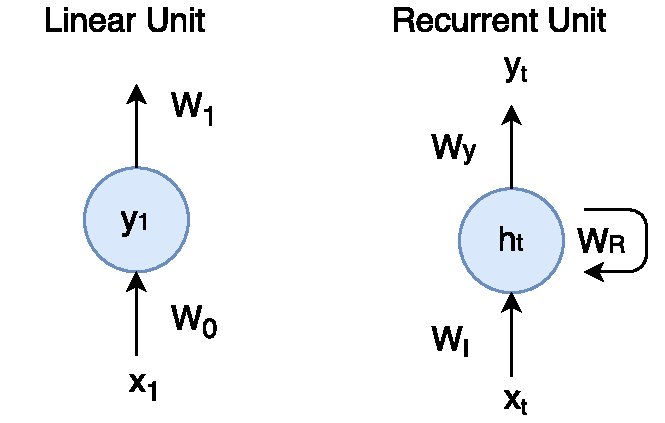
\includegraphics[width=0.5\textwidth]{Figures/RecurrentUnit}
	\caption{Linear vs. Recurrent unit}
	\label{Units}
\end{figure}
A linear unit's output is the input $x_{j}$ times the weight matrix $W_{ij}$ which is then passed to an activation function $g$.
\begin{equation}\label{linearOutput}
y_{i}=g(\sum_{j}W_{ij}x_{j}+b)
\end{equation}

The recurrent unit is composed of a linear unit, but then it adds a recurrent weight $W_{R}$, therefore the output $h^{(t)}$ depends on both the input $x_{t}$ and the activity at the previous time-step. To retrieve an output $y_{t}$ from the layer, a non linear activation function $g_{y}$ is applied to the $h^{(t)}$ \cite{NeonRNN}.
\begin{equation}\label{recurrentOutput}
\begin{aligned}
h^{(t)}&=g_{h}(W_{I}x^{(t)}+W_{R}h^{(t-1)}+b_{h})\\
y^{(t)}&=g_{y}(W_{y}h^{(t)}+b_{y})
\end{aligned}
\end{equation}

For example, in case of word prediction, the input of a unit can be a word, and the output of that unit would be the predicted next word that follows the one that was input; then, when the next input comes in at the next time-step, the process is applied, but also with the activity at the previous time-step taken into account.

The training of RNNs is different than that of the other ANNs, because RNNs emit an output at each time-step, and, therefore, there is a cost function at each time-step, whereas before, in feedforward networks, it was necessary to run the input through the whole network in order to get an output comparable to the one and only cost function. Another special characteristic of the RNNs is that the weights $W_{R}$ are shared across the network. So, the gradients from all the time-steps can be combined together to obtain the weights update and do back-propagation. But, because of the shared weights the update would scale with the size of the $W_{R}$, the back-propagation has to be done all the way until time-step zero, which causes the problem of vanishing and exploding gradients \cite{NeonRNN}.

In order to address the problems of training deep RNNs there are different solutions available. Among the known solutions are the use of the \textit{Root Mean Square Propagation} (RMSProp) optimizer for learning rate adjustment, clipping gradients, ReLu activation functions, special weight initialization, or to use \textit{gating} \cite{NeonRNN}. Gating is a technique for deciding when to forget the current input, and when to remember it for future time steps \cite{RNNvideo}. The most famous approaches are \textit{long short-term memory} (LSTM) and \textit{gated recurrent units} (GRU).

LSTM has at it's core a memory cell $C$ with a recurrent weight $W_{C}=1$ that inherits the activity of the previous time-step. This memory cell has three manipulations: \textit{forget} (flush the memory), \textit{input} (add to the memory), and \textit{output} (retrieve from the memory) \cite{NeonRNN}. The activity of the memory cell $C_{t}$ is taken and passed through a tanh activation function and multiplied by the \textit{gate}. The gate is an affine layer, or a 'standard' feedforward ANN layer, that has as inputs $x_{t}$ at the current time-step and $h_{t-1}$ of the previous time-step that are together multiplied by the weight $W_{0}$, summed and passed through the sigmoid activation function $\sigma$ to return a vector of numbers between $0$ and $1$. The gate operation for generating the \textit{output} $h_{t}$, or for getting the information from the memory cell $C_{t}$, is presented in the following equation:
\begin{equation}\label{gate}
\begin{split}
h_{t}&=\sigma(W_{0}\cdot \left [ x_{t} h_{t-1} \right ]+b_{0})\odot \textup{tanh}(C_{t})\\
&=o_{t}\odot \textup{tanh}(C_{t})
\end{split}
\end{equation}

The same approach is used for the \textit{forget} operation $f_{t}$. A layer before the final output is introduced, but with different weights, $W_{f}$. If the output of the forget gate is $0$, means that the memory has been flushed completely, whereas if the output is all $1$s then the memory retained everything \cite{NeonRNN}. The \textit{input} for the next time-step has two affine layers, one for generating new input $\widetilde{C_{t}}$ for the memory cell with the weights $W_{C}$ and tanh activation function, and another one $i_{t}$ that modulates the input and writes it into the memory cell with the weights $W_{i}$ and the sigmoid $\sigma$ activation function. All the components of the LSTM structure are vectors with numbers between $0$ and $1$, and they can be handled to perform either of the available manipulations. The summarized presentation of the LSTM components with the corresponding affine layers is illustrated in the Figure \ref{LSTMcore} \cite{NeonRNN}.
\begin{figure}[H]
	\centering
	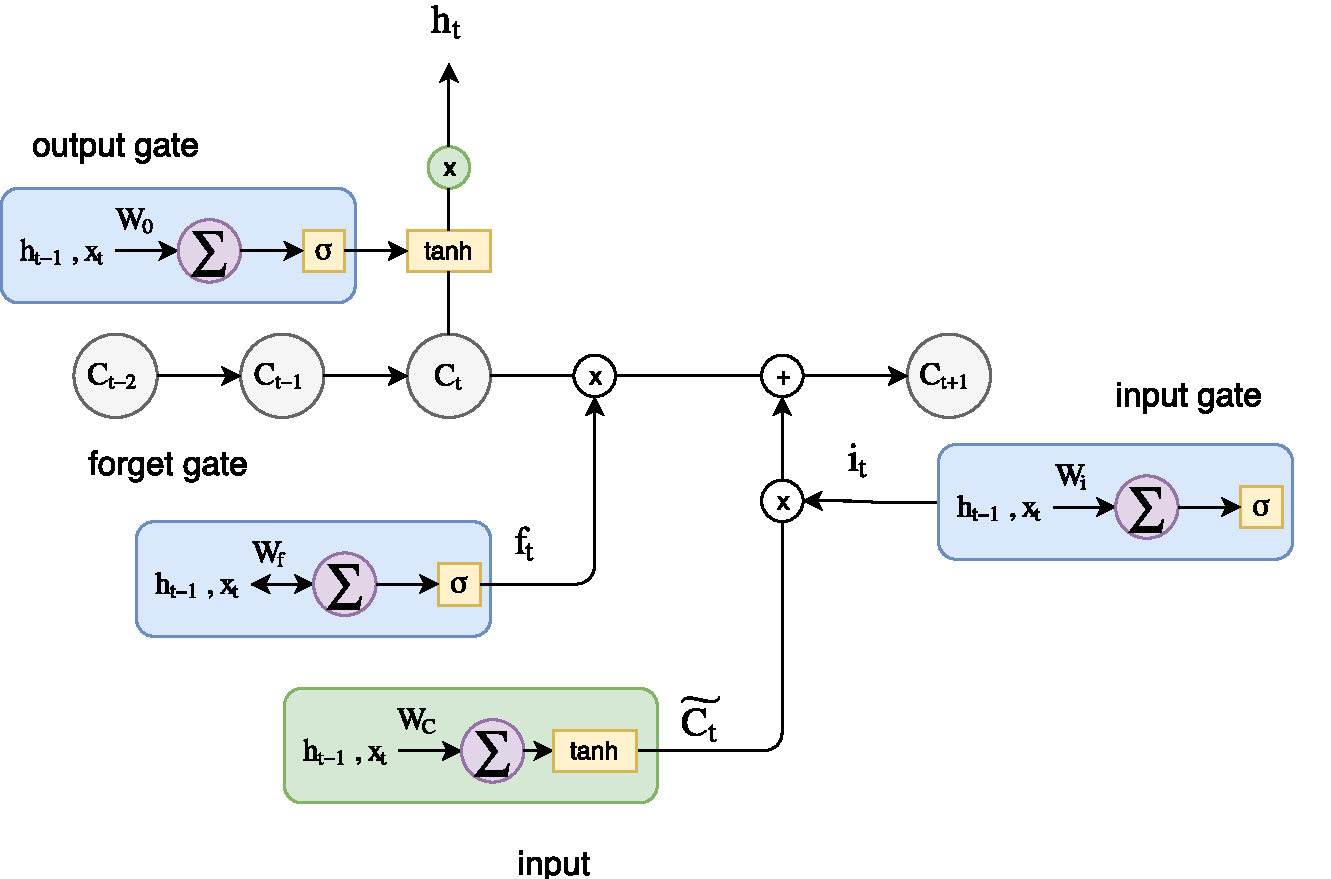
\includegraphics[width=0.9\textwidth]{Figures/LSTM}
	\caption{LSTM functionality}
	\label{LSTMcore}
\end{figure}

Having explained the LSTM functionality, the formula for computing the next time-step activity $C_{t+1}$ is the following:
\begin{equation}\label{LSTM}
C_{t+1}=f_{t}\odot C_{t}+i_{t}\odot \widetilde{C_{t}}
\end{equation}

The GRU gating approach is a simplified version of the LSTM. It actually combines all the gates into a single update:
\begin{equation}\label{GRU}
\begin{aligned}
h_{t}&=(1-z_{t})\cdot h_{t-1}+z_{t}\cdot \widetilde{h_{t}}\\
z_{t}&=\sigma(W_{z}\cdot[h_{t-1},x_{t}]) \textup{ (update gate)}\\
\widetilde{h_{t}}&=\textup{tanh}(W\cdot[r_{t}\cdot h_{t-1},x_{t}]) \textup{ (input gate)}\\
r_{t}&=\sigma(W_{r}\cdot[h_{t-1},x_{t}]) \textup{ (remember gate)}
\end{aligned}
\end{equation}

\subsubsection{Policy Gradient Methods} \label{PolicyGradMeths}
The \textit{Policy Gradient Methods} learn a \textit{parameterized policy} and makes it possible to select the action without calculating the value function. So, in a given state $s$, at a given time $t$, the agent selects an action $a$ based on the weights vector ${\theta}$ of the policy: ${\pi}(a|s,{\theta})=Pr\{A_{t}=a|S_{t}=s,{\theta}_{t}={\theta}\}$. The policy weights are learned according to an approximate gradient of a performance indicator ${\eta}({\theta})$ with respect to the policy weights, which tries to maximize the performance. All the methods of the form \Cref{gradM} are policy gradient methods:
\begin{equation}\label{gradM}
\theta_{t+1}=\theta_{t}+\alpha \nabla \eta (\theta_{t})
\end{equation}

The policy gradient methods are suitable for both \textit{discrete} and \textit{continuous} action spaces. For the discrete action space problems parameterized numerical preferences can be formed for each state-action pair, $h(s,a,\theta)$ \cite{Sutton}. The most preferred actions in each state have the highest probability of getting selected. The preferences can be parameterized randomly, for example, by being computed by a deep Q-network. The policy gradient theorem provides a formula for computing the gradient of the performance measure $\eta$ with respect to the policy weights vector $\theta$, composed of the state distribution $d_{\pi}(s)$, the state-action value function $q_{\pi}(s,a)$, and the gradient of the policy $\nabla_{\theta}\pi(a|s,\theta)$:
\begin{equation}\label{gradMTheorem}
\nabla\eta(\theta)=\sum_{a}d_{\pi}(s)\sum_{a}q_{\pi}(s,a)\nabla_{\theta}\pi(a|s,\theta)
\end{equation}

The methods that use both policy and value approximations are named \textit{actor-critic} methods, where the \textit{actor} estimates the policy weights vector for choosing an action and the \textit{critic} estimates the value weights for providing the information about the quality of a state the agent ends up in after making the action according to the policy. So, the actor is about the learned policy, and the critic - about the learned value function. 

There is an algorithm which is called \textit{reinforce} and it also uses both policy and value function approximation, but it doesn't bootstrap. The critic, on the other hand, is a bootstrapping critic, which updates it's states based on the value estimates of the next states. So, the initial reinforce algorithm has been changed for the actor-critic method: it's full return was replaced by one-step return. The one-step actor critic algorithm is presented below \cite{Sutton}.
\begin{algorithm}[H]
\caption{One-step Actor-Critic (episodic)}
\label{algo:AC}
\begin{algorithmic}
\State Input: differentiable policy parameterization $\pi(a|s,\theta),\forall a\in A, s\in S,\theta\in\mathbb{R}^{n}$
\State Input: differentiable state-value parameterization $\hat{v}(s,w),\forall s \in S, w \in \mathbb{R}_{m}$
\State Parameters: $\alpha>0,\beta>0$
\State Initialize policy weights $\theta$ and state-value weights $w$
\Repeat
\State Initialize $S$ (first state of episode)
\State $I\leftarrow 1$
\While{$S$ is not terminal}:
\State $A\sim \pi(\cdot|S,\theta)$
\State Take action $S$, observe $S'$, $R$
\State $\delta\leftarrow R+\gamma\hat{v}(S',w)-\hat{v}(S,w)$ (if $S'$ is terminal, then $\hat{v}(S',w)=0$)
\State $w\leftarrow w+\beta\delta\nabla_{w}\hat{v}(S,w)$
\State $\theta\leftarrow \theta+\alpha I \delta\nabla_{\theta} \textup{log} \pi(A|S,\theta)$
\State $I\leftarrow \gamma I$
\State $S\leftarrow S'$
\EndWhile
\Until forever
\end{algorithmic}
\end{algorithm}

As it was mentioned before, policy gradient methods work for discrete action spaces as well as for continuous. In the discrete actions problem, the policy is estimating the probability of each action in the discrete set. In the continuous actions space, on the other hand, the policy approximates the variance $\sigma^2$ and the mean $\mu$ of a normal distribution, which composes the probability distribution of the continuous actions. Therefore, the policy weight vector is composed of two elements, $\theta_{\mu}$ and $\theta_{\sigma}$ that can be used further in function approximation algorithms.